% !TEX TS-program = pdflatex

\documentclass[unicode,11pt,notheorems,xcolor=table]{beamer}

\usepackage[T2A]{fontenc}
\usepackage[utf8]{inputenc}
\usepackage[russian]{babel}
\usepackage{amsmath,amsfonts,amssymb,amsthm}
\usepackage{mathtools}
\usepackage{diagbox}

\usepackage{ulem}
\usepackage{tikz}
\usepackage{graphicx}
%\usepackage{tkz-graph}
\usetikzlibrary{matrix,arrows,decorations.pathmorphing, arrows.meta,positioning}
\usetikzlibrary{positioning,calc}
\usetikzlibrary{patterns}
\usetikzlibrary{decorations.pathreplacing}

%Описание стиля презентации
\usetheme[sidebar=0]{kfmn} 
\setbeamercovered{transparent}

%\definecolor{cyan}{RGB}{240,217,1}
%\definecolor{vgugreen}{RGB}{143,188,103}
%\definecolor{vgured}{RGB}{234,38,40}
%\definecolor{vgublue}{RGB}{53,101,167}
\hypersetup{colorlinks,linkcolor=,urlcolor=blue}

\makeatletter
	\g@addto@macro{\endtabular}{\rowfont{}}% Clear row font
	\makeatother
	\newcommand{\rowfonttype}{}% Current row font
	\newcommand{\rowfont}[1]{% Set current row font
		\gdef\rowfonttype{#1}#1\ignorespaces%
	}
\makeatother

\newcommand{\myunit}{9mm}
\tikzset{
    node style sp/.style={draw,circle,minimum size=\myunit},
    node style ge/.style={circle,minimum size=\myunit},
    arrow style mul/.style={draw,sloped,midway,fill=white},
    arrow style plus/.style={midway,sloped,fill=white},
}

%[0, 6, 8, 8, 10, 5, 6, 10, 8, 10, 10], 

\pgfdeclareimage[height=8mm]{university-logo}{logo-iem.png}
\logo{\pgfuseimage{university-logo}}
%2[0, 11, 10, 8, 11, 5, 11, 11, 8, 11, 10, 11],

\titlepicture{
	\begin{tikzpicture}[y=1.4cm,overlay,rotate=8]
	\coordinate (O) at (-3cm,0.9cm);
	\filldraw[thick,draw= vgublue, fill=vgublue!20!white] (0,0) circle[radius=4.2cm];
	\clip (0,0) circle[radius=4.2cm];
	\draw (-1.5,1.5) node{
	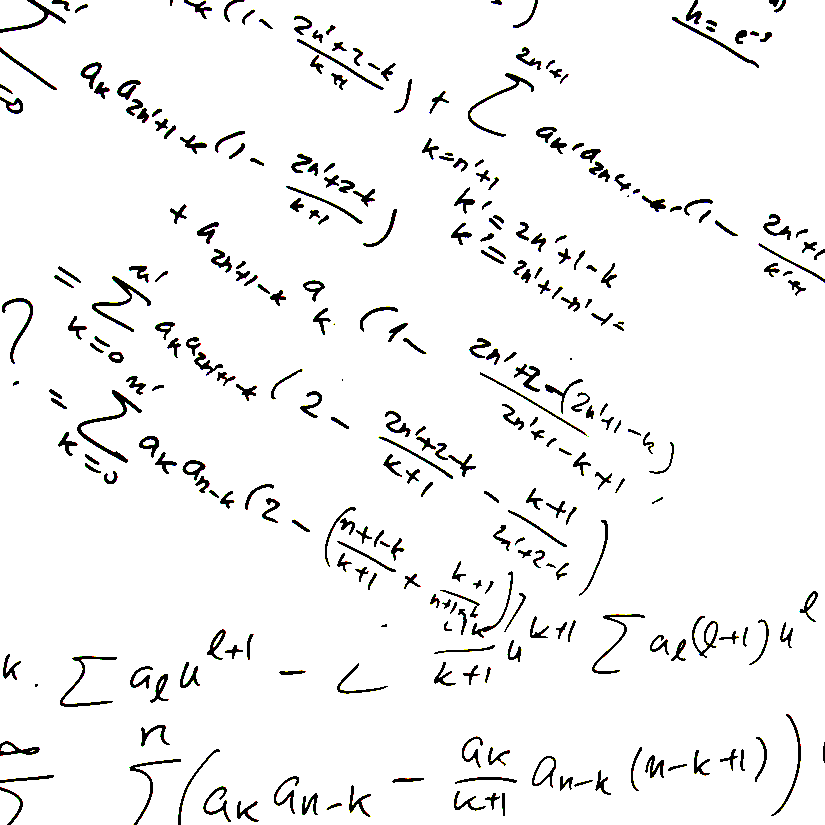
\includegraphics[width=8cm]{titlepic.png}
	};
\end{tikzpicture}
}

\usepackage[math]{iwona}

\newcommand{\hplus}{\mathbin{\hat+}}
\newcommand{\hdot}{\mathbin{\hat\cdot}}
% Описание теорем
\newtheorem{theorem}{Теорема}
\newtheorem{seq}{Следствие}
%%

\LECT % 

% Титульный лист теорем
\author[Д.\,В. Чупраков]{канд.\,физ.-матем.\,наук, доцент Д.\,В. Чупраков\\[6pt] usr10381@vyatsu.ru}

\institute[ВятГУ]{ФГБОУ ВО Вятский государственный университет}

\department{Факультет экономики и финансов}

\title[Лекция~15. Непрерывные случайные величины]{
	Введение в экономико-математическое моделирование\\[12pt]
	Лекция~15. Непрерывные случайные величины}
\date{9 декабря 2020~г.}


\setbeamercovered{invisible}

\setbeamercolor{math text}{fg=vgured!70!black}


\begin{document}


\maketitle

\begin{frame}{Структура лекции}{}
	\tableofcontents
\end{frame}

\section{Функции распределения и плотности распределения вероятностей}
\begin{frame}{}{}
    \begin{block}{Определение}
        Случайные величины, возможные значения которых непрерывно заполняют некоторый промежуток.
    \end{block}


    \bigskip
    Таблицу вероятностей построить невозможно.
    
    \bigskip
    \structure{Проблема:} 
    В каком виде представить закон распределения НСВ?  
    
    
    
\end{frame}

\begin{frame}{Функция распределения}{}
    \begin{block}{}
        Функция распределения вероятностей~--- это функция определенная на всей числовой прямой и принимающая значения, равные вероятности того, что случайная величина $X$ меньше наперед заданного числа $x$.
        $$
            F(x)=P(X<x)
        $$
        \end{block}
\end{frame}


\begin{frame}{События}{}
    $$
        P(X<a)=F(a), \qquad P(X \geqslant b) = 1-P(b)
    $$
    \begin{block}{}
        Вероятность того, что случайная величина $X$ примет значение, из полуинтервала $\left[ a,b\right)$ равнa разности функций распределения на его концах:
        $$
            P(a \leqslant X <b) = F(b)-F(a)
        $$
    \end{block}

    \vspace{-5mm}
    \begin{multline*}
        F(b) = P(X<b) 
        =\\
        = P(x<a)+ P(a \leqslant X <b) 
        =\\
        = F(a) + P(a \leqslant X <b)
    \end{multline*}
    % $$
    % P(a \leqslant X <b) = F(b)-F(a)
    % $$

\end{frame}

\begin{frame}{Практически невозможное событие}{}

    \begin{multline*}
        P(X=a) =  \lim_{\Delta x \to 0} P(a \leqslant X < a+\Delta x) 
        =\\
        = \lim_{\Delta x \to 0} (F(a+\Delta x) - F(a)) = F(a)-F(a)=0   
    \end{multline*}
    \begin{block}{}
        Вероятность того, что непрерывная случайная величина примет наперед заданное значение равна нулю.
        $$
        P(X=a)=0
        $$
    \end{block}

    
\end{frame}

\begin{frame}{Плотность распределения}{}
    \alert{Средней плотностью} распределения вероятностей называется отношение вероятности $Р(a<x<b)$  попадания случайной величины $x$ в тот или иной интервал $\Delta x$ ее значений к величине этого интервала: 
    $$
        \frac{p(a <x<b)}{b-a}
    $$
    \begin{block}{}
    Плотностью распределения $f(a)$ в точке $a$ называется предельное значение средней плотности.
    $$
        f(a) = \lim_{\Delta x \to 0} \frac{P(a\leqslant x < a+\Delta x)}{\Delta x} = \lim_{\Delta x \to 0} \frac{F(a+\Delta x)-F(a)}{\Delta x} = F'(a).
    $$
    \end{block}
\end{frame}

\begin{frame}{Функция плотности}{}
    \begin{block}{Функция плотности}
        Производная функции распределения характеризует плотность, с которой распределяется значение случайной величины в точке $x$ и называется \alert{функцией плотности}
        
        {\centering $ f(x) = F'(x) $  \par}
    \end{block}
    
    {\centering
        \includegraphics[width=8cm]{fx-1.png}    
    \par}
\end{frame}

\begin{frame}{События по функции плотности}{}
    {\centering
        \includegraphics[width=8cm]{fx-2.png}    
    \par}

    \vspace{-7mm}
    \begin{gather*}
        P(a \leqslant X < b) = \int\limits_a^b f(x)dx\\
        P(X < a) = \int\limits_{-\infty}^a f(x)dx\qquad \qquad\qquad\qquad
        P(X \geqslant b) = \int\limits_b^{+\infty}f(x)dx
    \end{gather*}
\end{frame}

\begin{frame}{Свойства плотности}{}
    {\centering
        \includegraphics[width=8cm]{fx-2.png}    
    \par}

    \vspace{-7mm}
    \begin{itemize}
        \item $\displaystyle f(x) \geqslant 0$ 
        \item $\displaystyle \lim_{x \to -\infty} f(x) = \lim_{x \to +\infty} f(x) =0$
        \item $\displaystyle \int\limits_{-\infty}^{+\infty} f(x)dx = 1 $
    \end{itemize}
\end{frame}

\begin{frame}{Связь между $f(x)$ и $F(x)$}{}
\begin{itemize}
    \item Вычисление плотности по функции распределения
    $$
        f(x)=F'(x)
    $$
    \item Вычисление функции распределения по плотности
    $$
        F(x) = \int\limits_{-\infty}^x f(t)dt
    $$
\end{itemize}
\end{frame}

\begin{frame}{Пример}{}

    \begin{exampleblock}{Пример}
        По функции распределения вычислить функцию плотности
        $$
            F(x) = \begin{cases}
                0, & x\leqslant 0\\
                x^2, & 0<x\leqslant 1\\
                1, &  x>1
        \end{cases}
        $$
    \end{exampleblock}

    \vspace{-6mm}
    \begin{align*}
        x & < 0 & F'(x) &=(0)' = 0\\
        0 &<x< 1  & F'(x) &= (x^2)'=2x \\
        1 &> x  & F'(x) &= (1)'=0 
    \end{align*}

    \vspace{-8mm}
    $$
    f(x) = \begin{cases}
        0, & x\leqslant 0\\
        2x, & 0<x\leqslant 1\\
        0, &  x>1
    \end{cases}
    $$
\end{frame}


\begin{frame}{График функции распределения}{}
    \begin{minipage}{6.5cm}
        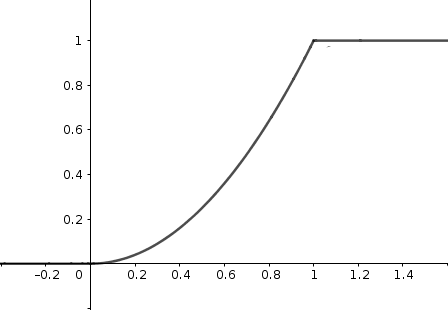
\includegraphics[width=6cm]{fx-example-1.png}
    \end{minipage}
    \begin{minipage}{4cm}
    $$ F(x) = \begin{cases}
        0, & x\leqslant 0\\
        x^2, & 0<x\leqslant 1\\
        1, &  x>1
    \end{cases}
    $$        
    \end{minipage}
\end{frame}

\begin{frame}{График плотности распределения}{}
    \begin{minipage}{6.5cm}
        \includegraphics[width=6cm]{fx-example-2.png}
    \end{minipage}
    \begin{minipage}{4cm}
    $$f(x) = \begin{cases}
        0, & x\leqslant 0\\
        2x, & 0<x\leqslant 1\\
        0, &  x>1
    \end{cases}
    $$        
    \end{minipage}
\end{frame}

\begin{frame}[allowframebreaks]{Пример}{}
    \begin{exampleblock}{Задача}
        Задана функция распределения вероятностей непрерывной случайной величины:
        $$F(x) = \begin{cases}
            0, & x\leqslant 0\\
            cx^2, & 0<x\leqslant 2\\
            1, &  x>2
        \end{cases}
        $$        
        Найти: 
        \begin{itemize}
            \item значение $c$
            \item функцию плотности распределения вероятностей $f(x)$, 
            \item вероятность попадания случайной величины $X$ в интервал $(0;1)$.         
        \end{itemize}
    \end{exampleblock}
    \framebreak
    \structure{Найдем плотность $f(x)$}
    $$
    f(x) = \begin{cases}
        0, & x< 0\\
        2cx, & 0<x< 2\\
        0, &  x>2
    \end{cases}
    $$        

    \structure{Вычислим $c$} из условия $\int_{-\infty}^{\infty} f(x)=1$
    \begin{multline*}
        1 = \int_{-\infty}^{+\infty} f(x) 
        =\\
         = \int_{-\infty}^0 0dx + \int_{0}^2 2cx dx + \int_2^{+\infty} 0dx  
         =\\
         = \int_{0}^2 \frac{cx}{2} dx
        = \left. cx^2 \right|_0^2 = 4c 
    \end{multline*}
    Итак, $4c=1$ или $c= \frac{1}{4}$.

    \framebreak
    \structure{Выпишем функции}
    $$
        F(x) = \begin{cases}
            0, & x\leqslant 0\\
            \frac{x^2}{4}, & 0<x\leqslant 2\\
            1, &  x>2
        \end{cases}
        \qquad
        f(x) = \begin{cases}
            0, & x< 0\\
            \frac{x}{2}, & 0<x< 2\\
            0, &  x>2
        \end{cases}
    $$ 
    
    \structure{Вычислим вероятность}
    $$
        P(0<X<1) = F(1)-F(0) = \frac{1^2}{4}-0 = \frac{1}{4}
    $$

\end{frame}
\section{Числовые характеристики непрерывной случайной величины}

\begin{frame}{Числовые характеристики}{}
    \begin{itemize}
        \item Медиана
        $$
            Me(X)=m, \qquad F(m)=1-F(m)=\frac{1}{2}
        $$
        \item Математическое ожидание
        $$
            M(X)= \int_{-\infty}^{+\infty} xf(x)dx
        $$
        \item Дисперсия
        $$
            D(X)= \int_{-\infty}^{+\infty} (x-M(x))^2 f(x)dx
        $$
        $$
            D(X)= M\big(X^2\big)-\big( M(x) \big)^2
        $$
        \item Среднее квадратическое отклонение
        $\sigma(X) =\sqrt{D(x)}$
    \end{itemize}
\end{frame}

\begin{frame}[allowframebreaks]{Пример}{}
    \begin{exampleblock}{}
        Найти числовые характеристики функции распределения:
        $$
        F(x) = \begin{cases}
            0, & x\leqslant 0\\
            \frac{x^2}{4}, & 0<x\leqslant 2\\
            1, &  x>2
        \end{cases}
        $$
    \end{exampleblock}
    \begin{itemize}
        \item Медиана 
        $$\begin{gathered}
            F(x)=\frac{1}{2}    \\
            \frac{x^2}{4} = \frac{1}{2}\\
            x^2=2\\
            x=\sqrt{2}
        \end{gathered}
        $$
        \item Вычислим функцию плотности:
        $$
        f(x) = \begin{cases}
            0, & x< 0\\
            \frac{x}{2}, & 0<x< 2\\
            0, &  x>2
        \end{cases}
        $$
        \item Математическое ожидание
        \begin{multline*}
            M(X)= \int_{-\infty}^{+\infty} xf(x)dx
            =\\
            = \int_{-\infty}^0 x0dx + \int_{0}^2 \frac{x^2}{2} dx + \int_2^{+\infty} x0 dx  
             =\\
             = \int_{0}^2 x^2 dx
            = \left. \frac{x^3}{6} \right|_0^2 = \frac{8}{6} =\frac{4}{3}
        \end{multline*}



        \item Дисперсия
        \begin{multline*}
            D(X)= \int_{-\infty}^{+\infty} (x-M(X))^2f(x)dx
            =\\
            = \int_{-\infty}^0 0dx + \int_{0}^2 \left(x-\frac{4}{3}\right)^2 \frac{x}{2} dx + \int_2^{+\infty} 0 dx  
             =\\
             \int_{0}^2 \left( \frac{x^3}{2} -\frac{4}{3}x^2 +\frac{8}{9}x \right)dx
             =\\
             =\left. \left( \frac{x^4}{8} -\frac{4}{9}x^3 +\frac{4}{9}x^2 \right)\right|_{0}^{2}
            = \left(\frac{2^4}{8} -\frac{4}{9}2^3 +\frac{4}{9}2^2\right) - 0
            =\\
            = \frac{2}{9}
        \end{multline*}

        \item Среднее квадратическое отклонение
        $$
            \sigma(X) =\sqrt{D(x)}= \frac{\sqrt{2}}{3}
        $$
    \end{itemize}
\end{frame}



\begin{frame}{Типы распределенией}{}
    \begin{itemize}
        \item равномерное распределение;
        \item нормальное (гауссово) распределение
    \end{itemize}
\end{frame}
\subsection{Равномерный закон распределения}
\section{Нормальный закон распределения}
\begin{frame}{Равномерный закон распределения}{}
    \begin{block}{Определение}
        Непрерывная случайная величина $X$ имеет \alert{равномерное распределение} на отрезке $[a,b]$, если ее плотность вероятности на этом отрезке постоянна, а вне отрезка $[a,b]$ равна 0:        
        $$
            f(x) = 
            \begin{cases}
                c & x \in [a,b]\\
                0 & x \notin [a,b]
            \end{cases}
        $$
    \end{block}
\end{frame}

\begin{frame}{Вычисление коэффициента}{}
    {\centering
        \includegraphics[width=8cm]{fx-3.png}
    \par}
 $$
    c \cdot(b-a) = 1, \qquad c=\frac{1}{b-a}
 $$
 $$
    f(x) = 
    \begin{cases}
        \dfrac{1}{b-a} & x \in [a,b]\\
        0 & x \notin [a,b]
    \end{cases}
    \qquad
    F(x) = 
    \begin{cases}
        0 & x < a\\
        \dfrac{x-a}{b-a} & a\leqslant x \leqslant b\\
        1 & x >b
    \end{cases}
$$
\end{frame}

\begin{frame}{Числовые характеристики}{}
    {\centering
        \includegraphics[width=9cm]{fx-3.png}
    \par}
 $$
    M(X) = \frac{b+a}{2} \qquad D(X)= \frac{(b-a)^2}{12}
 $$

\end{frame}
\begin{frame}[t]{Пример}{}
    \begin{exampleblock}{Задача}
         Найти  функцию распределения величины $X$, равноерно распределенной на отрезке $[2,4]$ и числовые характеристики этой величины.
    \end{exampleblock}
\end{frame}

\begin{frame}{Нормальное распределение}{}
    \begin{block}{Определение}
        Случайная величина $X$ подчиняется \alert{нормальному распределению $N(\mu,\sigma)$}, если ее плотность определена формулой:
        $$
            f (x) = \frac{1}{\sigma \sqrt{2\pi}} e^{\tfrac{(x-\mu)^2}{2\sigma^2}}
        $$
    \end{block}
    Нормальное распределение однозначно задается двумя параметрами:
    \begin{itemize}
        \item $\mu$~--- математическое ожидание,
        \item $\sigma$~--- среднее квадратическое отклонение.
    \end{itemize}

    \begin{block}{}
    Закон применим, когда на случайную  величину действует множество различных независимых факторов, каждый из которых в отдельности не имеет преобладающего значения.
    \end{block}
\end{frame}
\begin{frame}{График плотности}{}
    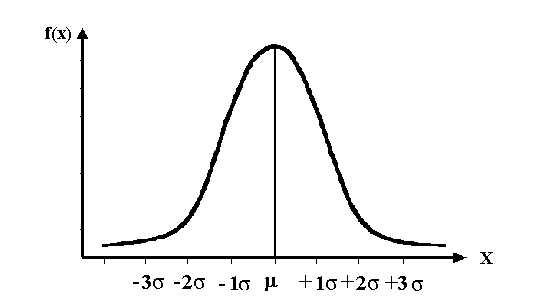
\includegraphics[width=10cm]{N-1.png}
\end{frame}
\begin{frame}{Закономерности}
    \begin{block}{}
        Параметр $\mu$ характеризует математическое ожидание случайной величины, являясь центром распределения и наиболее вероятным значением. 
    \end{block}
    \begin{itemize}
        \item Изменение $\mu$ не влияет на форму кривой, а только вызывает ее смещение вдоль оси $x$. 
        \item График нормальной кривой Гаусса симметиричен относительно прямой $x=\mu$.
        \item По мере увеличения разности $|x-\mu|$ значение $f(x)$ убывает. 
        \item При $(x-\mu)\to \infty$ значение $f(x)$ стремится к нулю, но никогда его не достигает. 
    \end{itemize}
    
\end{frame}
\begin{frame}{Закономерности}
    \begin{block}{}
        Параметр $\sigma$ характеризует изменчивость случайной величины 
    \end{block}
    \begin{itemize}
    \item  Чем больше $\sigma$, тем больше кривая растянута. 
    \item 
        \structure{Правило трех сигм} $\displaystyle P(|X-\mu| < 3\sigma )> 0.997$
    \end{itemize}
\end{frame}

\begin{frame}{Функция  распределения вероятностей}
    $$
        F(x) = \frac{1}{\sigma \sqrt{2\pi}} \int\limits_{-\infty}^x
    e^{\tfrac{(t-\mu)^2}{2\sigma^2}}dt 
    $$        

    \begin{block}{Вычисление}
        $$
        F(x) = \frac{1}{2}+ \Phi \left(\frac{x-\mu}{\sigma}\right)
        $$
    \end{block}
    где $\Phi(x)$~--- вычисляется по таблице функции Лапласа
    $$
    \Phi(x) = \frac{1}{\sqrt{2\pi}} \int\limits_0^x
    e^{\tfrac{x^2}{2}}dt 
    $$

\end{frame}

\begin{frame}{Классические задачи}
    \begin{block}{Вероятность попасть в промежуток}
        Вероятность того, что величина $X\sim N(\mu,\sigma)$ примет значение из $[a,b]$ равна
        $$
        P(a\leqslant X \leqslant b) = F(b)-F(a) = \Phi \left( \frac{b-\mu}{\sigma}\right)- \Phi \left( \frac{a-\mu}{\sigma}\right)
        $$
    \end{block}
    \begin{block}{Вероятность отклонения} 
        Вероятность того, что величина $X\sim N(\mu,\sigma)$ отклонится от своего математического ожидания не более чем на $\Delta$:
        $$
        P(|X-\mu| \leqslant \Delta = 2 \Phi \left( \frac{\Delta}{\sigma}\right)
        $$
    \end{block}

\end{frame}


\begin{frame}[t]{Пример}
    \begin{block}{}
        Магазин продает мужские костюмы. По данным статистики, распределение по размерам является нормальным с математическим ожиданием и средним квадратическим отклонением, соответственно равным 48 и 2. Определить процент спроса на костюмы 50-го размера при условии разброса значений этого размера в интервале (49, 51).
    \end{block}
\end{frame}
\begin{frame}[t]{Пример}
    \begin{block}{}
        Считается, что изделие~--- высшего качества, если отклонение его размеров от номинальных не превосходит по абсолютной величине 3.6~мм. Случайные отклонения размера изделия от номинального подчиняется нормальному закону со средним квадратическим отклонением, равным 3~мм. Систематические отклонения отсутствуют. Определить среднее число изделий высшего качества среди 100 изготовленных.
    \end{block}
\end{frame}
\begin{frame}[t]{Пример}
    \begin{block}{}
        Для некоторой величины $X$ известно, что $P(X<1)=0.5$, $P(-2\leqslant X\leqslant 4)=0.9973$. Предполагая, что величина распределена нормально найти ее Математическое ожидание и среднее квадратическое отклонение.
    \end{block}
\end{frame}

% \begin{frame}[t]{Пример}
%     Величина имеет математическое ожидание $6$ и среднее квадратическое отклонение $2$. Считая величину $X$ нормально распределенной случайной величиной, найти множество ее значений.
% \end{frame}
\end{document}
